\documentclass[11pt,a4paper]{article}

\usepackage[margin=0.5in, top=3cm, bottom=2cm]{geometry}
\usepackage[spanish, activeacute]{babel}
\usepackage[utf8]{inputenc}
\usepackage{amsthm}
\usepackage{amsmath}
\usepackage{amsfonts}
\usepackage{amssymb}
\usepackage{graphicx} %Para incluir el logo de la UBA
\usepackage{caratula} %Para armar el cuadro de integrantes
\usepackage{todonotes}
\usepackage{float}
\usepackage[lined,ruled,linesnumbered]{algorithm2e}
\usepackage{hyperref}
\usepackage{xcolor}
\usepackage[final]{pdfpages}
\providecommand{\DontPrintSemicolon}{\dontprintsemicolon}

\graphicspath{{imagenes/}}

\newcommand\comentario[2]{\textbf{{[#1: \textcolor{red}{#2}}}]}
\renewcommand\comentario[2]{}

\setcounter{secnumdepth}{5}

\begin{document}

\integrante{Almansi, Emilio}{674/12}{ealmansi@gmail.com}
\integrante{Fixman, Martín}{391/11}{martinfixman@gmail.com}
\integrante{Gunski, María Celeste}{899/03}{celestegunski@gmail.com}
\integrante{Maurizio, Miguel}{635/11}{miguelmaurizio\_92@hotmail.com}

\def\Materia{Bases de Datos}
\def\Titulo{Trabajo Pr\'{a}ctico 2}
\def\Fecha{1er Cuatrimestre 2016}
%----- CARATULA -----%

\thispagestyle{empty}

\begin{center}
	
\includegraphics[scale = 0.25]{imagenes/logo_uba.jpg}
\end{center}

\begin{center}
	{\textbf{\large UNIVERSIDAD DE BUENOS AIRES}}\\[1.5em]
	{\textbf{\large Departamento de Computaci\'{o}n}}\\[1.5em]
    {\textbf{\large Facultad de Ciencias Exactas y Naturales}}\\
    \vspace{35mm}
    {\LARGE\textbf{\Materia}}\\[1em]    
    \vspace{15mm}
    {\Large \textbf{\Titulo}}\\[1em]
    \vspace{15mm}
    {\textbf{\Large \Fecha}}\\
    \vspace{15mm}
    \textbf{\tablaints}
\end{center}

\newpage
\thispagestyle{empty}
\tableofcontents

\parskip=5pt
\setlength{\parindent}{0pt}

\newpage
\setcounter{page}{1}
\pagenumbering{arabic}
\pagestyle{plain}

\section{Introducci'on}

Las bases de datos relacionales SQL cuentan con muchas ventajas pero su utilización puede ser imposible en el caso de tener grandes volúmenes de datos. En cambio, las bases de datos NoSQL tienen la principal ventaja de manejar mucha más inforcación debido a la posibilidad de escalar en forma horizontal, lo cual no es posible con las bases de datos tradicionales. Es decir, para aumentar la cantidad de datos que procesa una base de datos relacional debemos tener una computadora mejor. 

Por otro lado, al estar utilizando una base NoSQL se puede incrementar la capacidad mediante una mayor cantidad de computadoras. Esto implica que en contextos donde la cantidad de datos aumenta rápidamente debemos utilizar una arquitectura distribuida, forzándonos a usar una base de datos NoSQL. 

En este trabajo estudiamos la bases de datos NoSQL. Particularmente aquellas de la familia orientada a documentos, utilizando la tecnología $MongoDB$.

En la primera parte, utilizando el problema del trabajo práctico 1, estudiamos y analizamos el diseño de los documentos a utilizar con el propósito de responder queries específicas. No solo creamos la base SQL, sino que también implementamos la migración de SQL a NoSQL.


En la segunda parte, utilizamos el esquema $Map$ $Reduce$ para realizar consultas sobre los datos, permitiendo parelelismo en su ejecución.


Por último, exploramos e investigamos la técnica de \textit{sharding}.

\newpage
\section{Parte 1}
Para el dise\~no de la base de documentos solicitada se tomar\'a como base la siguiente porci\'on del modelo realizado para el Trabajo Pr\'actico nro. 1\footnote{Cabe aclarar que se han quitado las FK a entidades que no aparecen en la porci\'on que estamos utilizando, para darle mayor claridad a la lectura}:

\begin{description}
\item[Usuario](\underline{idUsuario}, calle, numero, localidad, telefono, email, tipo)\\
PK=\{idUsuario\}

 \item[SuscripcionRubiOriente](\underline{idSuscripcion}, periodo, \dashuline{idUsuario})\\
PK=\{idSuscripcion\}\\
FK=\{idUsuario\}

 \item[Factura](\underline{idFactura}, periodo, monto, \dashuline{idUsuario})\\
PK=\{idFactura\}\\
FK=\{idUsuario\}

\item[Publicacion](\underline{idPublicacion}, titulo, fecha, precio, \dashuline{tipoPublicacion}, tipoVigencia, tipoVenta, \dashuline{idUsuario})\\
PK=\{idPublicacion\}\\
FK=\{tipoPublicacion, idUsuario\}

 \item[PublicacionFinalizada](\underline{\dashuline{idPublicacion}})\\
PK=\{idPublicacion\}\\
FK=\{tipoPublicacion\}

 \item[TipoPublicacion](\underline{nombre}, comision, costo, nivel, caducidad)\\
PK=\{nombre\}

 \item[Item](\underline{idItem}, \dashuline{idPublicacion}, nombre, tipo)\\
PK=\{idItem\}\\
FK=\{idPublicacion\}

 \item[Producto](\underline{\dashuline{idItem}})\\
PK=\{idItem\}\\
FK=\{idItem\}

 \item[Servicio](\underline{\dashuline{idItem}}, precioXHora)\\
PK=\{idItem\}\\
FK=\{idItem\}

 \item[Compra](\underline{idCompra}, fecha, \dashuline{idUsuario}, \dashuline{idPublicacion}, \dashuline{idCalificacion})\\
PK=\{idCompra\}\\
FK=\{idUsuario, idPublicacion, idCalificacion\}

 \item[Calificacion](\underline{idCalificacion}, valoracionComprador, valoracionVendedor, comentarioComprador, comentarioVendedor)\\
PK=CK=\{idCalificacion\}

\end{description}

que se corresponde con la secci\'on del diagrama que vemos a continuaci\'on

\begin{landscape}
    \begin{figure}[c]
        \frame{\includegraphics[scale=0.40]{imagenes/der-tp2.png}}
        \captionof{figure}{Diagrama Entidad Relaci\'on}
    \end{figure}
\end{landscape}

Desnormalizando esta porci\'on del modelo, generamos los dise\~nos de la base de documentos solicitada:

\begin{itemize}
\item Los documentos correspondientes a las facturas enviadas tendr\'an el siguiente dise\~no:
\begin{verbatim}
{"id","usuario","suscripcionRubi","monto","fecha"}
\end{verbatim}
Los datos para llenarlos se pueden obtener ejecutando la siguiente consulta en la base de SQL:
\begin{verbatim}
SELECT f.idFactura AS id, f.idUsuario AS usuario, 1 AS suscripcionRubi, f.monto, 
f.periodo AS fecha
FROM factura f 
INNER JOIN suscripcionRubiOriente sr ON f.idUsuario = sr.idUsuario
WHERE f.periodo = sr.periodo 
AND f.periodo < date('now','-1 month')
UNION 
SELECT f.idFactura AS id, f.idUsuario AS usuario, 0 AS suscripcionRubi, f.monto, 
f.periodo AS fecha
FROM factura f
WHERE f.idUsuario NOT IN 
(SELECT idUsuario FROM suscripcionRubiOriente WHERE periodo = f.periodo)
AND f.periodo < date('now','-1 month')
\end{verbatim}

\item Los documentos correspondientes a las ventas realizadas tendr\'an el siguiente dise\~no:
\begin{verbatim}
{"id","fecha","idComprador","idVendedor","calificacionComprador",
  "calificacionVendedor","comision","tipoPublicacion"}
\end{verbatim}
Los datos para llenarlos se pueden obtener ejecutando la siguiente consulta en la base de SQL:
\begin{verbatim}
SELECT c.idCompra AS id, c.fecha AS fecha, c.idUsuario AS idComprador,
p.idUsuario AS idVendedor, cal.valoracionComprador AS calificacionComprador, 
cal.valoracionVendedor AS calificacionVendedor, (tp.comision * p.precio) AS comision, 
"servicio" AS tipoDePublicacion
FROM compra c, calificacion cal, publicacion p, publicacionFinalizada pf, 
tipoPublicacion tp, item it
WHERE c.idPublicacionFinalizada = pf.idPublicacion AND pf.idPublicacion = p.idPublicacion 
AND p.nombreTipoPublicacion = tp.nombre 
AND it.idPublicacion = c.idPublicacionFinalizada AND it.tipo = 1
AND c.idCalificacion = cal.idCalificacion
AND c.fecha < date('now','-1 month')
UNION
SELECT c.idCompra AS id, c.fecha AS fecha, c.idUsuario AS idComprador, 
p.idUsuario AS idVendedor, cal.valoracionComprador AS calificacionComprador, 
cal.valoracionVendedor AS calificacionVendedor, 
(tp.comision * p.precio) AS comision, "producto" AS tipoDePublicacion
FROM compra c, calificacion cal, publicacion p, publicacionFinalizada pf, 
tipoPublicacion tp, item it
WHERE c.idPublicacionFinalizada = pf.idPublicacion AND pf.idPublicacion = p.idPublicacion 
AND p.nombreTipoPublicacion = tp.nombre 
AND it.idPublicacion = c.idPublicacionFinalizada AND it.tipo = 0
AND c.idCalificacion = cal.idCalificacion
AND c.fecha < date('now','-1 month')
UNION
SELECT c.idCompra AS id, c.fecha AS fecha, c.idUsuario AS idComprador, 
p.idUsuario AS idVendedor, cal.valoracionComprador AS calificacionComprador, 
cal.valoracionVendedor AS calificacionVendedor, 
(tp.comision * p.precio) AS comision, "mixto" AS tipoDePublicacion
FROM compra c, calificacion cal, publicacion p, publicacionFinalizada pf, 
tipoPublicacion tp, item it
WHERE c.idPublicacionFinalizada = pf.idPublicacion AND pf.idPublicacion = p.idPublicacion 
AND p.nombreTipoPublicacion = tp.nombre 
AND it.idPublicacion = c.idPublicacionFinalizada AND it.tipo <> 0 AND it.tipo <> 1
AND c.idCalificacion = cal.idCalificacion
AND c.fecha < date('now','-1 month')
\end{verbatim}

\end{itemize}

\newpage
\section{Ejercicio 2}

En la sección previo desnormalizamos la base de datos SQL. En esta parte vamos a realizar diversas consultas utilizando $Map$ $Reduce$.

\subsection{Importe total de ventas por usuario}

Por cada factura registrada, vemos el usuario y el importe, luego calculamos el total paralelizando por usuario: \\

\begin{verbatim}
var map1 = function(){
    emit(this["id"],this["monto"])
}

var reduce1 = function(key,values){
    return Array.sum(values)
}
\end{verbatim}

\subsection{reputación histórica de cada usuario}
Por cada venta devolvemos tanto el puntaje del comprador como del vendedor. Luego juntamos todas las calificaciones en un mismo nodo.


Entendemos que la $reputacion$ $historica$ se refiere al promedio de las calificaciones. Si fuera otra la función, no sería un problema dado que tenemos el historial completo de cada usuario en cada reduce y podríamos implementar otra diferente.

\begin{verbatim}
var map2 = function(){
    emit(this["idComprador"],this["calificacionComprador"])
    emit(this["idVendedor"],this["calificacionVendedor"])
}

var reduce2 = function(key,values){
    return Array.sum(values) / values.length
}
\end{verbatim}

\subsection{Operaciones con comisión más alta}

En este caso debemos saber cuál es el valor de la comisión más alta, la forma que encontramos para resolver es enviar todas las operaciones (en realidad solo el id y la comisión) a un solo nodo y ahi calcular las oeraciones con comisión máxima.

\begin{verbatim}
var map3 = function(){
    var pair = {"comision": this["comision"], "id": this["id"]};
    emit(0, pair)
}

var reduce3 = function(key,values){
    var max = 0;
    for(var i =0; i < values.length; i++){
        max = Math.max(max, values[i]["comision"]);
    }
    res = [];
    for(var i =0; i < values.length; i++){
        if(values[i]["comision"] === max) {
            res.push(values[i]["id"])
        }
    }	
    return {"res": res};
}
\end{verbatim}

\subsection{Monto total facturado por año}

Revisamos las facturas, separamos por año y luego sumamos cada monto. Notemos que el reduce es solamente sumar, que es lo mismo que usamos en el reduce de la consulta 1.

\begin{verbatim}
var map4 = function(){
    var s = new Date(
                this["fecha"].replace( /(\d{2})\/(\d{2})\/(\d{4})/, "$2/$1/$3")
            ).getFullYear();
    emit(s, this["monto"]);
}

var reduce4 = reduce1
\end{verbatim}

\subsection{Monto total facturado por año con suscripción Rubí}

Esta consulta es idéntica a la consulta 4, con la diferencia que antes de emitir en el map debemos chequear que en la factura tenga suscripción a Rubí del oriente.

\begin{verbatim}
var map5 = function(){
    if(this["suscripcion"] === "Rubí"){
        var s = new Date(
                this["fecha"].replace( /(\d{2})\/(\d{2})\/(\d{4})/, "$2/$1/$3")
            ).getFullYear();
        emit(s, this["monto"])		
    }
}

var reduce5 = reduce1

\end{verbatim}

\subsection{Total publicaciones por tipo}

Revisamos las ventas y emitimos el tipo, luego contamos cuantas aparecen de cada una.

\begin{verbatim}
var map6 = function(){
    emit(this["tipoPublicacion"], 1)		
}

var reduce6 = reduce1

\end{verbatim}

\newpage
\section{Parte 3}

El proceso de Sharding consiste en guardar una base de datos a través de muchas máquinas. Esta es la forma en la que MongoDB provee una alternativa para soportar escalabilidad en casos donde la cantidad de datos o el volúmen de pedidos sobre la base excede a las capacidades de una única máquina, mecanismo conocido como "horizontal scaling".

En particular, MongoDB provee dos estrategias de sharding que difieren en su forma de distribuir los registros de datos a través de las distintas máquinas disponibles en función del valor de un atributo dado de los documentos, definido como la clave.

\begin{itemize}
  \item Sharding por range: los datos comienzan almacenados en una única máquina, y a medida que crece el volúmen de datos se mantiene una estadística del rango donde están contenidos todos los valores del atributo clave de los registros que fueron insertados. Cuando el tamaño del primer shard supera un determinado umbral, se realiza una partición en el espacio de las claves y se distribuyen equitativamente los registros.
  \item Sharding por hashing: ante la inserción de un nuevo documento, se aplica una función hash sobre el atributo clave, luego determinando a partir del resultado cuál será el número de shard correspondiente para el nuevo registro. Se busca generalmente que la función de hash distribuya los datos uniformemente, de forma tal que un nuevo documento tenga una probabilidad de aproximadamente $\frac{1}{\#shards}$ de ser asignado a cada shard.
\end{itemize}

En general, cualquier base de datos de gran volúmen y/o pedidos que cuente con un atributo propicio para actuar de clave es un potencial caso de uso para sharding. Si adicionalmente los registros poseen una partición natural que podría beneficiarse al ser alojados en distintas máquinas, los incentivos son aún mayores. Un ejemplo de esto podría ser una base de datos de usuarios divididos por regiones (ej, clientes de latinoamérica, clientes de Europa, clientes de Asia). Otros casos típicos son bases de datos de entidades numeradas o con identificadores numéricos como libros identificados por su ISBN, o vehículos distribuídos según su TAN.

\subsection{Experimentación y consideraciones}

Configuramos una instalación de MongoDB en modo Sharding, con un total de 5 shards locales (es decir, 5 procesos ejecutándose en una misma máquina, pero funcionando autónomamente como si se encontraran en distintos dispositivos). En el caso de ambas estrategias de sharding, realizamos un experimento consistente en insertar 500.000 documentos en una colección en modo sharding, midiendo cada 20.000 inserciones el estado actual de los shards activos.

En una primera instancia, repetimos el experimento diez veces con sharding en modo range, y en segundo lugar, lo repetimos diez veces en modo hashed. El estado observado luego de cada iteración de 20.000 inserciones fue la cantidad total de documentos almacenados en cada shard.

Como clave para el proceso de sharding, fue elegido un id entero arbitrario tomado de forma aleatoria y sin repetición en el intervalo 0 ... 500.000. Esta elección respeta los lineamientos generales para obtener buena performance a partir de la elección de clave\footnote{https://docs.mongodb.com/manual/tutorial/choose-a-shard-key/}: el espacio de claves es divisible efectivamente (entre dos claves cualquieras, es sencillo definir el rango de claves que están en medio de ellas), y adicionalmente las claves tienen una distribución uniforme dentro del espacio permitido (ninguna parte del espacio de claves es más densa que otra).

\subsection{Resultados}

En primer lugar, mostramos la progresión en los tamaños de los distintos shards en función de la cantidad de iteraciones. Esto permite analizar la distribución de datos entre los distintos shards, y hasta qué punto la misma es uniforme. Esto se puede observar en las figuras \ref{fig:publicaciones-ranges} y \ref{fig:publicaciones-hashed}.

\begin{figure}[h!]
  \centering
  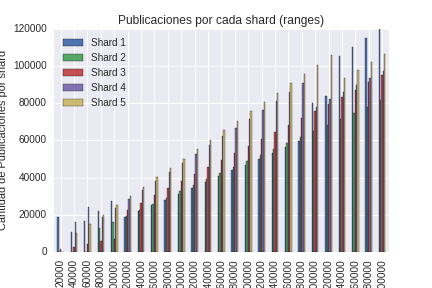
\includegraphics[width=4in]{imagenes/publicaciones_by_shard_ranges.png}
  \caption{Cantidad de documentos por shard (ranges).}
  \label{fig:publicaciones-ranges}
\end{figure}

\begin{figure}[h!]
  \centering
  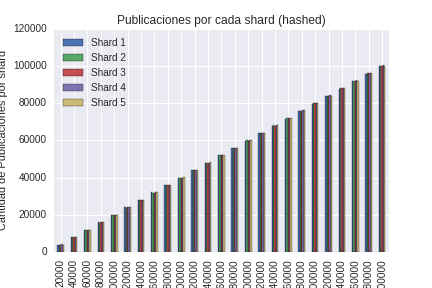
\includegraphics[width=4in]{imagenes/publicaciones_by_shard_hashed.png}
  \caption{Cantidad de documentos por shard (hashed).}
  \label{fig:publicaciones-hashed}
\end{figure}

Al inspeccionar las figuras, se observa cómo efectivamente los datos se distribuyen entre los distintos shards, dado que la cantidad de documentos almacenados en cada shard crece linealmente con el tamaño total de la colección.

Notablemente, la distribución en el caso de sharding por hashing es prácticamente ideal. La función de hash aplicada sobre todos los elementos de un conjunto aleatorio uniforme presenta en mayor medida una distribución aleatoria uniforme.

El comportamiento en el caso de sharding por rangos no muestra la misma uniformidad. Luego de la primera tanda de inserciones, casi el 100\% de los documentos se encuentran almacenados en el primer shard. A partir de la segunda tanda, se comienzan a utilizar todos los shards pero con una distribución fuertemente sesgada hacia los shards 1 y 4. A medida que la cantidad de documentos es mayor, la distribución muestra una estructura más regular y más homogénea, aunque siempre con un fuerte sesgo hacia el shard 1.

El hecho de que el comportamiento de la distribución con sharding por rangos sea más errático durante las primeras tandas de inserciones, se explica con el hecho de que, al comenzar el experimento, MongoDB no tiene información alguna sobre la distribución o los rangos de las claves de los documentos que se ingresarán a la base. A medida que se realizan más inserciones, la estimación en tiempo real de MongoDB es cada vez más precisa respecto al rango verdadero del set de claves, permitiendo una mejor distribución de los documentos entre los distintos shards.

\newpage
\section{Conclusi'on}

En este trabajo estudiamos los modelos de bases de datos no relacionales. Hemos realizado un diseño en el paradigma $document$ $oriented$ pensado para optimizar querys particulares,  donde luego utilizamos la técnica de MapReduce. También utilizamos $sharding$ para que en un escenario hipotético los accesos a los datos sean eficientes. Se puede observar que el modelado de las bases NoSQL es sencillo y permite que las consultas sean mas simples que en las tradicionales SQL ya que el diseño se orienta a responder consultasde nuestro interes.\\

Tanto MapReduce como Sharding ponen en evidencia la capacidad de estas bases para un escenario de cómputo distribuido, en los cuales los datos se encuentran en varias computadoras.\\

En particular observamos que sharding, bajo ciertas hipotesis en la distribucion de datos ingresados, puede balancear la carga de datos en distintos nodos. Esto supone una mejor utilización del hardware e incluso un mejor tiempo de respuesta para el usuario.

\newpage

\end{document}
